%ex14.tex

\section{Exercice 14 - Coloration de Sommets}\label{ex14}

\begin{center}
\begin{algorithm}[H]
\caption{Approximation de $\chi$(G) s\'equentielle}\label{ex14_algo}
\algsetup{indent=2em,linenodelimiter= }
\begin{algorithmic}[1]
\REQUIRE $G$ : graphe de n sommets
\ENSURE $\chi(G)$ : nombre de couleurs n\'ecessaires pour colorer G
\STATE Soit $x_1,...,x_n$ une num\'erotation des sommets de G.
\STATE Soit $C = \{1,2,...,k\}$ un ensemble de couleurs.
\FORALL {$x_i$}
	\STATE $\chi(G) = min\{k \in C : \forall y \in voisinage(x_i), \chi(y) \neq k\}$
\ENDFOR
\RETURN $\chi(G)$
\end{algorithmic}
\end{algorithm}
\end{center}

\subsection{Question 1}\label{ex14_q1}
Soit la num\'erotation suivante (parcours en profondeur \`a partir du premier sommet) :
%ex14_fig1.tex
%numerotation de l'exemple

\begin{figure}[h]
	\begin{center}
	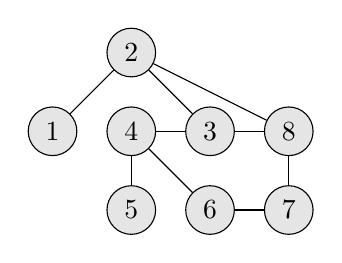
\begin{tikzpicture}
		\node[circle,draw=black,fill=black!10] (x1) at (0,0) {1};
		\node[circle,draw=black,fill=black!10] (x2) at (1,1) {2}
			edge[-] (x1);
		\node[circle,draw=black,fill=black!10] (x3) at (2,0) {3}
			edge[-] (x2);
		\node[circle,draw=black,fill=black!10] (x4) at (1,0) {4}
			edge[-] (x3);
		\node[circle,draw=black,fill=black!10] (x5) at (1,-1) {5}
			edge[-] (x4);
		\node[circle,draw=black,fill=black!10] (x6) at (2,-1) {6}
			edge[-] (x4);
		\node[circle,draw=black,fill=black!10] (x7) at (3,-1) {7}
			edge[-] (x6);
		\node[circle,draw=black,fill=black!10] (x8) at (3,0) {8}
			edge[-] (x3)
			edge[-] (x2)
			edge[-] (x7);
	\end{tikzpicture}
	\end{center}
	\caption{Exemple de numérotation}
	\label{ex24_fig1}
\end{figure}



En appliquant l'algorithme ci-dessus on obtient la coloration suivante :
%ex14_fig2.tex
%coloration via l'algo de l'exemple


On remarque que sur cet exemple, la solution est optimale : $\chi(G) = 3$.

\subsection{Question 2}\label{ex14_q2}
Malheureusement la solution renvoy\'ee n'est pas toujours tr`es bonne, en effet il est
possible de construire un graphe 2-colorable pour lequel l'algorithme renverra
$\frac{n}{2}$.

En effet, soient les graphe bipartis $G = (V,E)$ suivants :\\
\begin{itemize}
	\item $V = \{1,2,...,n\}$ ;
	\item $E = \{(i,j) \forall i,j \in V : i\ impair,\ j\ pair,\ et\ j \neq i+1\}$
\end{itemize}

%ex14_fig3.tex
%coloration via l'algo 

\begin{figure}[H]
	\begin{center}
	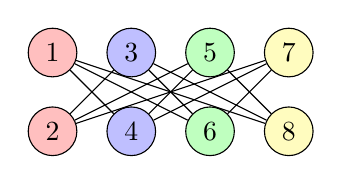
\begin{tikzpicture}
		\node[circle,draw=black,fill=red!25] (x1) at (0,0) {1};
		\node[circle,draw=black,fill=blue!25] (x3) at (1,0) {3};
		\node[circle,draw=black,fill=green!25] (x5) at (2,0) {5};
		\node[circle,draw=black,fill=yellow!25] (x7) at (3,0) {7};
		\node[circle,draw=black,fill=red!25] (x2) at (0,-1) {2}
			edge[-] (x3)
			edge[-] (x5)
			edge[-] (x7);
		\node[circle,draw=black,fill=blue!25] (x4) at (1,-1) {4}
			edge[-] (x1)
			edge[-] (x5)
			edge[-] (x7);
		\node[circle,draw=black,fill=green!25] (x6) at (2,-1) {6}
			edge[-] (x1)
			edge[-] (x3)
			edge[-] (x7);
		\node[circle,draw=black,fill=yellow!25] (x8) at (3,-1) {8}
			edge[-] (x1)
			edge[-] (x3)
			edge[-] (x5);
	\end{tikzpicture}
	\end{center}
	\caption{Coloration par l'algorithme}
	\label{ex24_fig3}
\end{figure}



En ex\'ecutant l'algorithme sur un tel graphe, on voit rapidement que le nombre de
couleurs utilis\'ees sera bien \'egal au nombre de sommets divis\'e par deux.
Sur l'exemple de la figure, on voit que pour $n = 6$, la solution $\chi_{alg}(G_{fig3}) =
3$ tandis que $\chi_{opt}(G_{fig3}) = 2$.

%ex14_fig1.tex
%coloration optimale

\begin{figure}[h]
	\begin{center}
	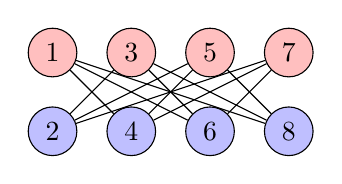
\begin{tikzpicture}
		\node[circle,draw=black,fill=red!25] (x1) at (0,0) {1};
		\node[circle,draw=black,fill=red!25] (x3) at (1,0) {3};
		\node[circle,draw=black,fill=red!25] (x5) at (2,0) {5};
		\node[circle,draw=black,fill=red!25] (x7) at (3,0) {7};
		\node[circle,draw=black,fill=blue!25] (x2) at (0,-1) {2}
			edge[-] (x3)
			edge[-] (x5)
			edge[-] (x7);
		\node[circle,draw=black,fill=blue!25] (x4) at (1,-1) {4}
			edge[-] (x1)
			edge[-] (x5)
			edge[-] (x7);
		\node[circle,draw=black,fill=blue!25] (x6) at (2,-1) {6}
			edge[-] (x1)
			edge[-] (x3)
			edge[-] (x7);
		\node[circle,draw=black,fill=blue!25] (x8) at (3,-1) {8}
			edge[-] (x1)
			edge[-] (x3)
			edge[-] (x5);
	\end{tikzpicture}
	\end{center}
	\caption{Coloration optimale}
	\label{ex24_fig4}
\end{figure}



